%% ============================================================
%%  SBEG108 – Numerical Methods in Biomedical Engineering
%%  Spring 2026 · Cairo University · Dr. Muhammad Rushdi
%%
%%  Official IEEE Conference Template (Error-Free & Customized)
%% ============================================================
\documentclass[9pt, conference]{IEEEtran}

%% ---------- Standard Layout & Packages ----------
\usepackage[top=0.65in, bottom=0.65in, left=0.62in, right=0.62in]{geometry}
\usepackage{cite}
\usepackage{enumitem}
\setlist[itemize]{itemsep=0pt, topsep=2pt, parsep=0pt}
\usepackage{amsmath, amssymb,amsfonts}
\usepackage{algorithmic}
\usepackage{graphicx}
\usepackage{textcomp}
\usepackage{booktabs} 
\usepackage{caption}
\usepackage{cases}

\usepackage{float}
\floatplacement{figure}{H} 
\usepackage{etoolbox}
\font\captionfont=cmss10 at 8pt
\font\captionlabel=cmssbx10 at 8pt
\addtolength{\textfloatsep}{-20pt} 
\addtolength{\intextsep}{-20pt}
\addtolength{\floatsep}{-10pt}
\setlength{\abovecaptionskip}{2pt}
\setlength{\belowcaptionskip}{0pt}
\setlength{\abovedisplayskip}{3pt}
\setlength{\belowdisplayskip}{3pt}
\setlength{\abovedisplayshortskip}{1pt}
\setlength{\belowdisplayshortskip}{1pt}
%% ---------- Custom Colors & Interactivity ---------
\usepackage{xcolor}
\definecolor{ieeeblue}{RGB}{0,70,135} 
\definecolor{lightbg}{RGB}{240,244,248} 

\usepackage[
    colorlinks=true,
    linkcolor=ieeeblue,
    citecolor=ieeeblue,
    urlcolor=ieeeblue
]{hyperref}

%% ---------- Table & Figure Caption Color Styling ----------
\font\captionfont=cmss10 at 8pt
\font\captionlabel=cmssbx10 at 8pt
\captionsetup[table]{labelfont={bf,color=ieeeblue},textfont={it},tableposition=top,labelsep=period}
\captionsetup[figure]{labelfont={bf,color=ieeeblue},textfont={it},labelsep=period}

\begin{document}

%% -------- TITLE --------
\title{\fontfamily{phv}\selectfont\color{ieeeblue}\textbf{Numerical and Machine Learning Methods for the Diabetes Glucose Tolerance Test}}

% -------- AUTHORS, AFFILIATIONS & COURSE BANNER (All-in-One Safe Layout) --------
\author{
    \begin{tabular}{ccc}
        \parbox{2.1in}{\centering
            Aya Sayed Anwar\\
            Ganna Emad El-Din Salah\\
            Habiba Abdel-Moneim Ramadan\\
            Habiba Ahmed Farhat\\[1ex]
            
        } & 
        \parbox{2.1in}{\centering
            Jana Hazem Mohamed\\
            Jana Mostafa Mohamed\\
            Jana Waleed Abdel-Hamid\\
            Yassen Mohamed Ahmed\\[1ex]
        
        } & 
        \parbox{2.1in}{\centering
            Maryam Mostafa Shaban\\
            Radwa Hamdy Hussein\\
            Suty Fady Zakaria\\[1ex]
        
        }
    \end{tabular}\\[1ex] % كسر السطر للنزول تحت الأسماء مباشرة
    % --- البار مدمج هنا لضمان ظهوره تحت الأسماء في الصفحة الأولى تماماً ---
    \normalfont\normalsize
    \colorbox{lightbg}{
      \parbox{0.96\textwidth}{\centering \footnotesize \color{ieeeblue} \textbf{SBEG108 Numerical Methods in Biomedical Engineering --- Course Project --- Spring 2026} \\ \textit{Under the Supervision of Dr. Muhammad Rushdi --- Cairo University}}
    }
}

\begin{document}

\maketitle

% هنا يبدأ نص التقرير مباشرة (مثال: \section{Introduction}) دون الحاجة لكتابة كود البار في الأسفل مجدداً

%% ============================================================
%%  ABSTRACT & KEYWORDS
%% ============================================================
\begin{abstract}
This report evaluates computational solutions for Randall's 2-ODE model to simulate a 12-hour Oral Glucose Tolerance Test (OGTT) across four metabolic scenarios. To address the system's non-linear feedback loops, we implement and contrast three strategies: a custom fixed-step RK4 method, an adaptive Dormand-Prince (RK45) scheme, and a Physics-Informed Neural Network (PINN). Benchmarks show that while fixed-step integration introduces discretization errors during sudden post-infusion spikes, the adaptive RK45 scheme efficiently balances precision with computational speed. Furthermore, the PINN framework successfully embeds physiological constraints to capture metabolic trends without grid dependencies, demonstrating strong potential for continuous glucose monitoring (CGM) systems.
\end{abstract}

\begin{IEEEkeywords}
Oral Glucose Tolerance Test, Randall Model, Runge-Kutta, Physics-Informed Neural Networks, Biomedical Simulation.
\end{IEEEkeywords}

%% ============================================================
%%  I. INTRODUCTION
%% ============================================================
\section{\color{ieeeblue}Introduction}
\IEEEPARstart{T}{he} Oral Glucose Tolerance Test (OGTT) is a critical diagnostic tool for evaluating pancreatic responsiveness, yet discrete blood draws fail to capture continuous physiological feedback loops. To bridge this gap, we implement Randall's 2-ODE model to simulate extracellular glucose $G(t)$ and insulin $I(t)$ dynamics over 12 hours. We benchmark three computational approaches to handle the system's non-linear, multi-scale nature: a custom fixed-step RK4 solver, an adaptive Dormand-Prince (RK45) scheme, and a Physics-Informed Neural Network (PINN). Our work analyzes the core trade-offs between classical numerical accuracy and modern learning-based techniques for real-time metabolic monitoring.

% TODO (Member 1 & 10): Expand motivation paragraph.

%% ============================================================
%%  II. LITERATURE REVIEW
%% ============================================================
\section{\color{ieeeblue}Literature Review}

This survey covers three pillars relevant to the project:
ODE modelling of glucose--insulin dynamics, physics-informed
and neural ODE methods for metabolic systems, and benchmarking
of numerical integration schemes.

\subsection{Coupled ODE Models of Glucose--Insulin Dynamics}

Kumnungkit et al.~\cite{kumnungkit2022} proposed a minimal
glucose--insulin ODE model incorporating food intake, achieving
$R^{2} > 0.99$ against both minimal and maximal reference models.
Their work confirms that low-dimensional coupled ODE systems can
capture clinically relevant dynamics without the identifiability
problems of high-dimensional compartmental models --- a philosophy
shared by the two-ODE system adopted in this project, where $G(t)$
and $I(t)$ are the sole state variables and the insulin effect
appears as the nonlinear term $-G_{g}\,I\,G$.

Aliffi et al.~\cite{aliffi2024} fitted stochastic ODE systems to
CGM data from eight type-2 diabetic subjects using Particle Swarm
Optimisation and information-theoretic model selection. They
demonstrate the limitations of the classical three-variable Schiesser (Randall) 2-ODE Model
formulation for OGTT data and support simpler two-state
representations, consistent with the model used here.

\subsection{Physics-Informed and Neural ODE Methods}

Wang et al.~\cite{wang2025pignn} introduced PIGNN, embedding
glucose--insulin ODE residuals directly into the network loss:
\begin{equation}
\color{ieeeblue}
  \mathcal{L} = \mathcal{L}_{\text{data}}
              + \lambda\,\mathcal{L}_{\text{physics}},
  \label{eq:pinn_loss}
\end{equation}
achieving $0.726 \pm 0.126$\,mmol/L accuracy on 52 subjects and
a $12.33\,\%$ improvement over data-driven baselines with only
48 training samples.

Pathirana et al.~\cite{pathirana2026} extended PINNs for
glucose--insulin digital twins using Federated Learning,
reporting a mean ODE residual of 0.033 and prediction errors
within $10$\,mg/dL, demonstrating that physics constraints
substantially improve robustness under sparse clinical data.

Kainth et al.~\cite{kainth2025pinode} introduced PI-NODE-SR,
combining a Heun solver with scale-aware residual normalisation
to stabilise Neural ODE training on stiff biophysical systems ---
directly relevant to the fast post-load glucose spike followed
by the slow insulin recovery phase characteristic of the OGTT.

\subsection{Benchmarking of Numerical Integration Schemes}

St\"{a}dter et al.~\cite{stadter2021} benchmarked ODE solvers
across biological models from the BioModels database, showing
that adaptive multi-step methods consistently outperform
fixed-step Runge--Kutta schemes on stiff systems in both accuracy
and wall-clock time. These findings motivate the fixed-step RK4
versus adaptive RK45 comparison conducted in this project.
% TODO (Member 9): Survey 5–8 papers published 2022–2026.

%% ============================================================
%%  III. ODE MODEL DESCRIPTION
%% ============================================================
\section{\color{ieeeblue}Mathematical Model \& Simulation Cases}

The Schiesser two-compartment ODE model~\cite{schiesser2014} simulates the Oral Glucose Tolerance
Test (OGTT) by tracking extracellular glucose $G(t)$ and insulin $I(t)$ over
12 hours. This model is based on the pioneering work of Randall~\cite{randall1980}. The glucose balance is governed by:

\begin{equation}
\color{ieeeblue}
\small
  C_g\,\frac{dG}{dt} =
  \begin{cases}
    Q + I_n - G_g\,I\,G - D_d\,G,        & G < G_k,\\[3pt]
    Q + I_n - G_g\,I\,G - D_d\,G - \mu(G-G_k),&G \ge G_k,
  \end{cases}
  \label{eq:glucose}
\end{equation}

where $Q$ is basal hepatic production, $I_n$ is the 30-minute oral glucose
infusion ($G_t=80{,}000$\,mg), $-G_g IG$ is insulin-mediated uptake,
$-D_d G$ is insulin-independent metabolism, and $-\mu(G-G_k)$ is renal
excretion active only above the threshold $G_k=250$\,mg/Ll.
Insulin evolves according to:

\begin{equation}
\color{ieeeblue}
\small
  C_i\,\frac{dI}{dt} =
  \begin{cases}
    -A_a\,I,                   & G < G_0,\\[3pt]
    -A_a\,I + B_b(G - G_0),    & G \ge G_0,
  \end{cases}
  \label{eq:insulin}
\end{equation}

where $-A_a I$ is first-order clearance and $B_b(G-G_0)$ is pancreatic
$\beta$-cell secretion triggered above $G_0=51$\,mg/dL. The system
starts at the fasting steady state $G(0)=81.14$, $I(0)=5.671$\,mg/dL.

The baseline model was originally implemented in R~\cite{rteam2024} using the \texttt{deSolve} \texttt{lsoda} solver~\cite{deSolve2010}. Four cases were simulated by varying the pancreatic sensitivity $B_b$:
a no-infusion baseline (Case~1), a normal OGTT (Case~2), reduced $B_b$
producing hyperglycemia, and increased $B_b$ causing hypoglycemia.

% ================================================================
%  Simulation Figures (4 Cases Results)
% ================================================================


\begin{figure}[!htbp]
    \centering
    \begin{minipage}[t]{0.48\columnwidth}
      \centering
      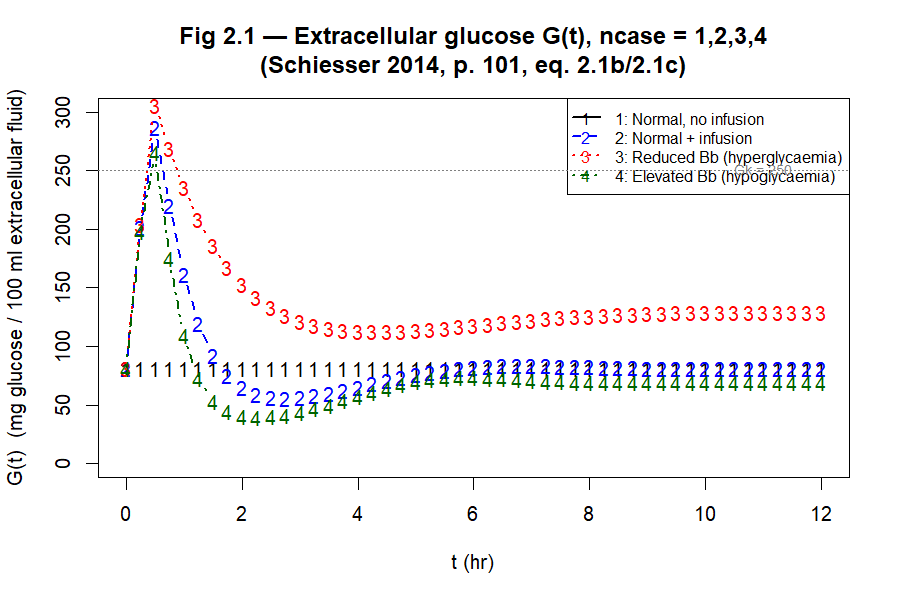
\includegraphics[width=\linewidth]{fig2_1_glucose_G.png}
      \caption{Extracellular glucose $G(t)$ across the four simulated cases.}
      \label{fig:glucose_G}
    \end{minipage}
    \hfill
    \begin{minipage}[t]{0.48\columnwidth}
      \centering
      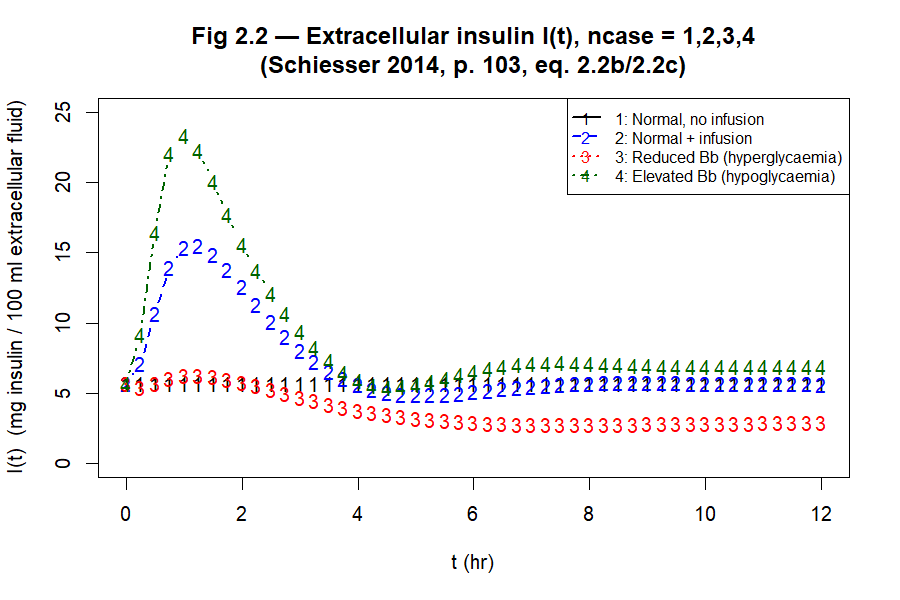
\includegraphics[width=\linewidth]{fig2_2_insulin_I.png}
      \caption{Plasma insulin $I(t)$ showing pancreatic response variations.}
      \label{fig:insulin_I}
    \end{minipage}
\end{figure}

\begin{figure}[!htbp]
    \centering
    \begin{minipage}[t]{0.48\columnwidth}
      \centering
      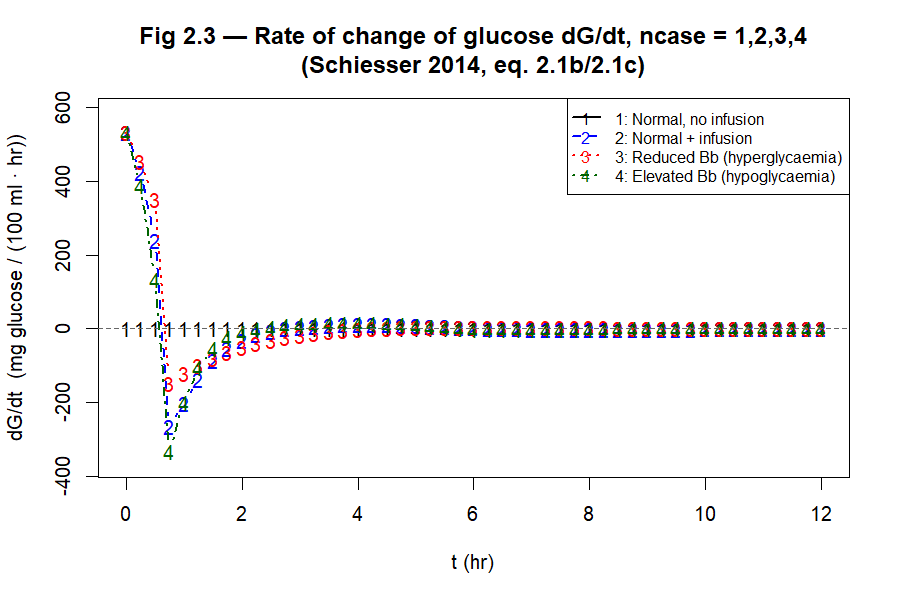
\includegraphics[width=\linewidth]{fig2_3_dGdt.png}
      \caption{Rate of change $dG/dt$, highlighting the sharp transient phase.}
      \label{fig:dGdt}
    \end{minipage}
    \hfill
    \begin{minipage}[t]{0.48\columnwidth}
      \centering
      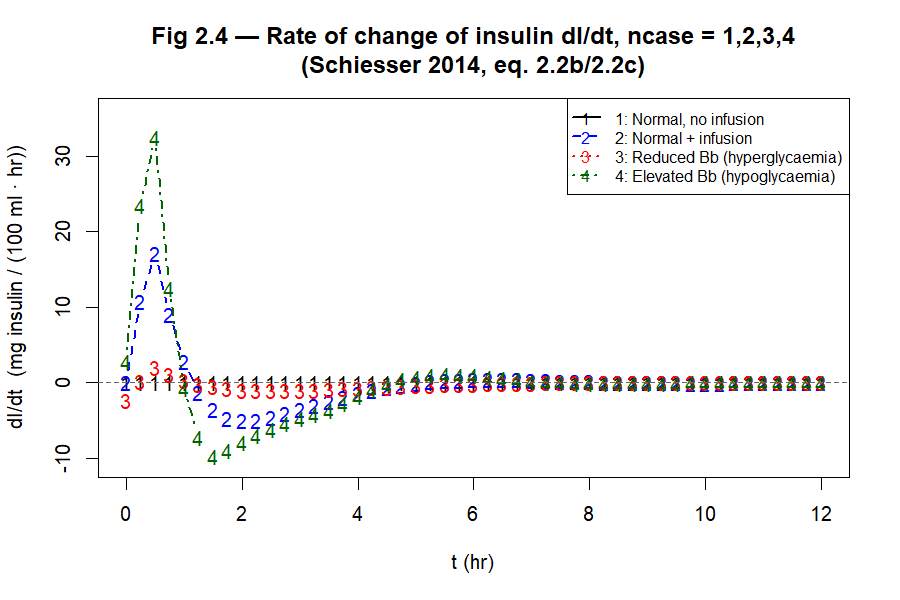
\includegraphics[width=\linewidth]{fig2_4_dIdt.png}
      \caption{Rate of change $dI/dt$, illustrating dynamic activation thresholds.}
      \label{fig:dIdt}
    \end{minipage}
\end{figure}



%% ============================================================
%%  IV. NUMERICAL SOLUTION – RK4
%% ============================================================
\section{\color{ieeeblue}Numerical Solution -- RK4}

The coupled nonlinear ordinary differential equations describing the glucose-insulin homeostatic loop during an OGTT lack analytical solutions, requiring numerical approximation. In this study, the classical fourth-order Runge-Kutta (RK4) method was implemented as a numerical baseline. RK4 achieves fourth-order local accuracy by computing a weighted average of four intermediate derivative evaluations within each integration step.

For a general initial value problem:
\begin{equation}
\color{ieeeblue}
\small
\frac{dy}{dt} = f(t,y)
\label{eq:ivp}
\end{equation}
\noindent the state vector is updated simultaneously via:
\begin{equation}
\color{ieeeblue}
\small
y_{n+1} = y_n + \frac{h}{6}(k_1 + 2k_2 + 2k_3 + k_4)
\label{eq:rk4_update}
\end{equation}
\noindent where $h$ represents the step size, and the intermediate slopes are evaluated sequentially as:
\begin{align}
\small
\color{ieeeblue}
k_1 &= f(t_n, y_n) \\
\color{ieeeblue}
k_2 &= f\left(t_n + \frac{h}{2}, y_n + \frac{h}{2}k_1\right) \\
\color{ieeeblue}
k_3 &= f\left(t_n + \frac{h}{2}, y_n + \frac{h}{2}k_2\right) \\
\color{ieeeblue}
k_4 &= f(t_n + h, y_n + h k_3)
\end{align}

\noindent A convergence analysis (Fig.~\ref{fig:rk4_convergence}) shows that the global order drops to 1--2 due to three model discontinuities: glucose infusion termination ($t = 0.5\text{ h}$), renal threshold ($G = 250\text{ mg/dL}$), and pancreatic threshold ($G = 51\text{ mg/dL}$). However, in the smooth late-time region ($t \in [6,12]\text{ h}$), the theoretical fourth-order behavior recovers with a rate of 4.04.

\begin{figure}[!htbp]
    \centering
    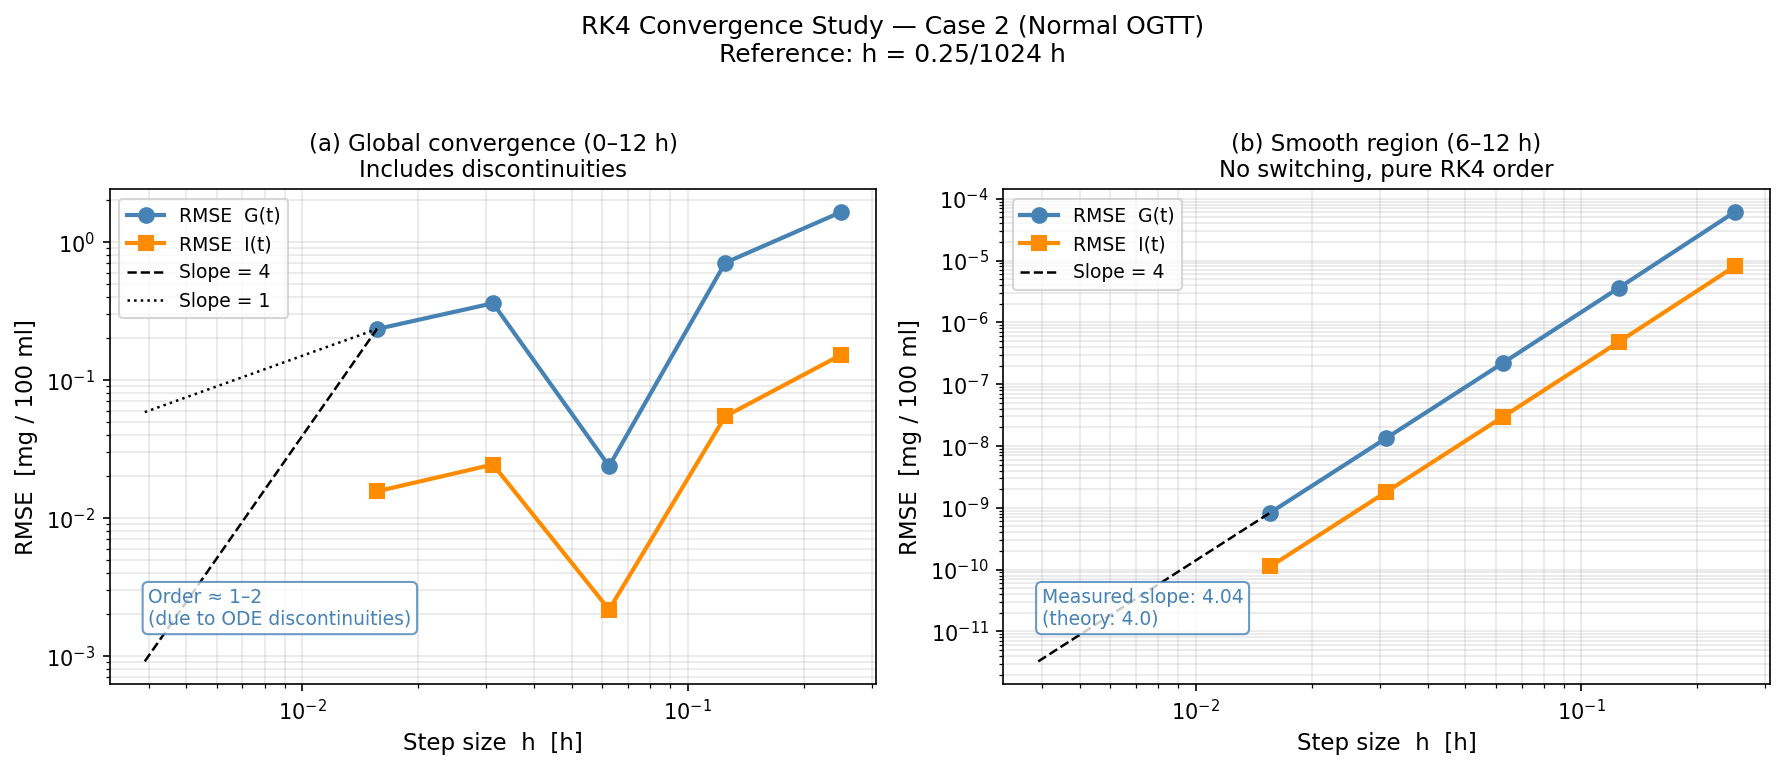
\includegraphics[width=0.25\textwidth]{rk4_convergence_fixed.png}
    \caption{RK4 convergence study for Case 2 (Normal + OGTT) showing the RMSE for glucose $G(t)$ and insulin $I(t)$ profiles compared against the theoretical slope = 4 reference line.}
    \label{fig:rk4_convergence}
\end{figure}

% TODO (Member 4): State RK4 update rule.

%% ============================================================
%%  V. NUMERICAL SOLUTION – ADAPTIVE RK45
%% ============================================================
\section{\color{ieeeblue}Numerical Solution -- Adaptive RK45}
While fixed-step RK4 is inefficient for multi-scale physiological systems, the adaptive-step Runge-Kutta-Fehlberg (RK45) method optimizes efficiency for the Oral Glucose Tolerance Test (OGTT). The OGTT features rapid non-linear transient spikes in the first 30 minutes, followed by a slow 11.5-hour basal decay. Utilizing the Dormand-Prince algorithm, RK45 computes embedded fourth and fifth-order approximations of $G(t)$ and $I(t)$. Thanks to the First Same As Last (FSAL) property, this requires only six function evaluations per step. The step-size $h$ is dynamically adjusted based on the local truncation error ($ee$); it shrinks during rapid transient phases to preserve accuracy and expands during stable decay. Consequently, RK45 minimizes total integration steps and significantly reduces CPU wall-clock time while maintaining high clinical accuracy.


%% ============================================================
%%  VI. MACHINE LEARNING SCHEME – PINN
%% ============================================================
\section{\color{ieeeblue}Machine Learning Scheme (PINN)}

The simulation of Randall's two-ODE glucose--insulin model was executed
across a 12-hour domain ($T = 12\,\text{h}$) to evaluate the tracking
performance and stability of the implemented solvers.  A Physics-Informed
Neural Network (PINN) was subsequently trained on the same domain to
demonstrate that deep-learning surrogates can replace grid-based
integrators while strictly honouring the underlying physiology.

% ------------------------------------------------------------
\subsection{Numerical Solvers vs.\ PINN Evaluation}
% ------------------------------------------------------------

The transient behaviour of extracellular glucose $G(t)$ (mg/dL) and
plasma insulin $I(t)$ ($\mu$U/mL) during the 12-hour Oral Glucose Tolerance
Test (OGTT) was successfully captured by both the classical solver and the
PINN surrogate.  As illustrated in Fig.~\ref{fig:GI_comparison}, the sharp
non-linear spike triggered by the 30-minute oral glucose load is followed by
a prolonged, smooth basal decay toward the equilibrium state defined by
\begin{equation}
  G_{\infty} = 81.14\;\text{mg/dL}, \qquad I_{\infty} = 5.671\;\text{$\mu$U/mL}.
\end{equation}
\vspace{0.1cm}
\begin{figure}[H]
  \centering
  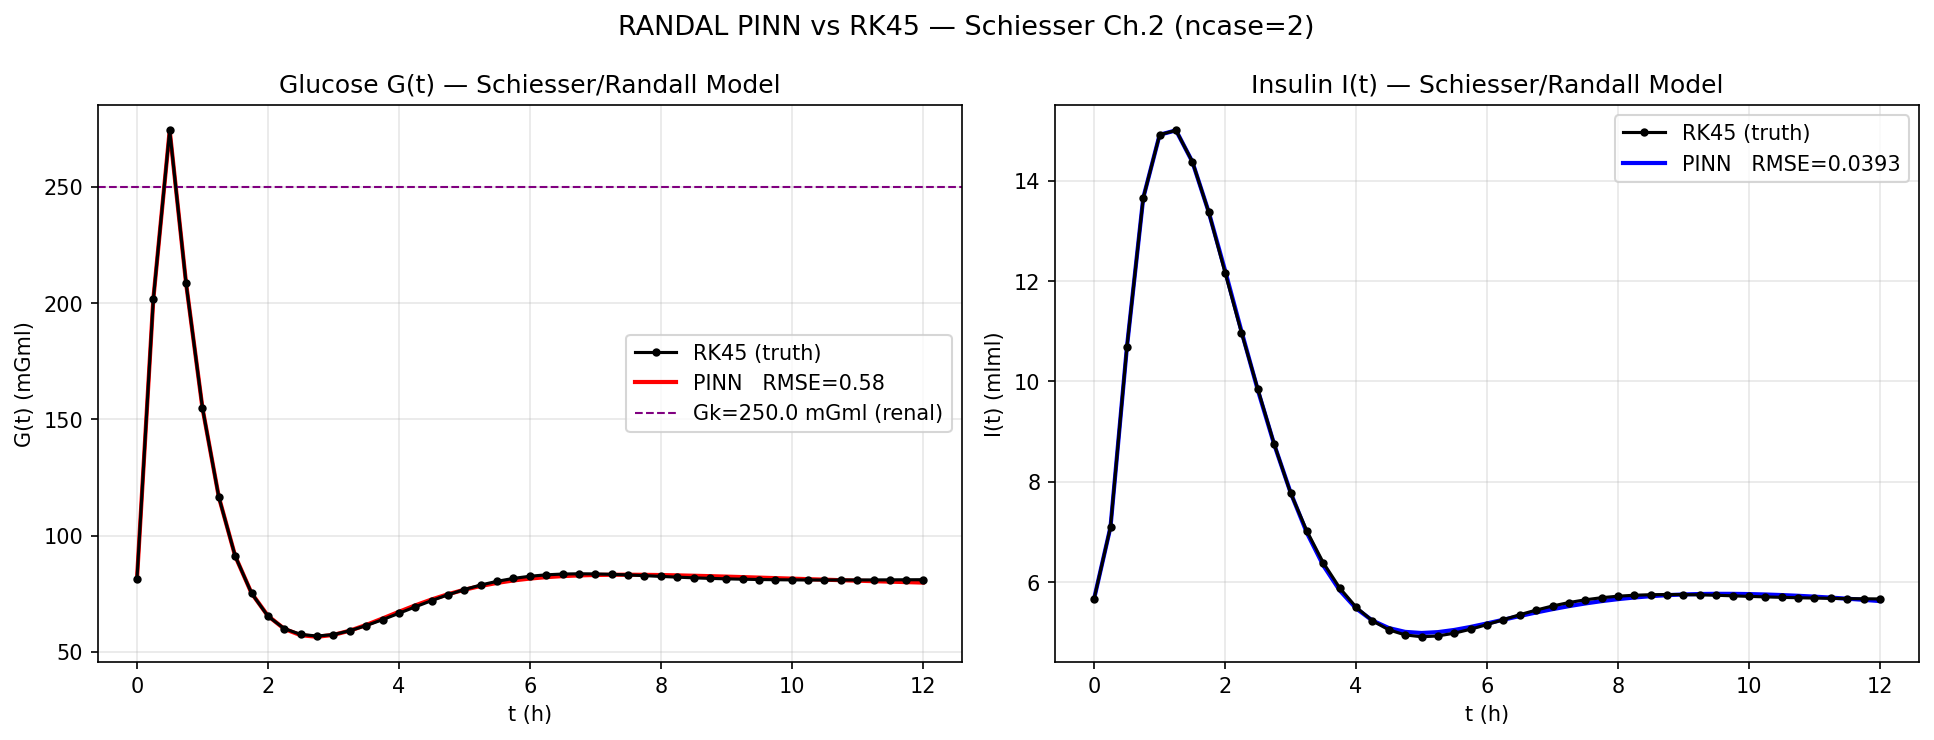
\includegraphics[width=0.82\columnwidth]{GI_comparison}
  \caption{Continuous 12-hour simulation of glucose $G(t)$ and insulin
           $I(t)$ levels tracking the non-linear physiological response
           during the OGTT load.  Black markers denote RK45 (ground truth);
           the coloured lines show the PINN predictions
           (RMSE$_G = 0.575$\,mg/dL, RMSE$_I = 0.039$\,$\mu$U/mL).}
  \label{fig:GI_comparison}
\end{figure}
\vspace{0.1cm}

The adaptive Dormand--Prince (RK45) scheme dynamically allocated smaller
step sizes during the volatile initial phase to maintain high local
precision, while automatically enlarging the step size $h$ during the slow
recovery phase to maximise computational throughput.

% ------------------------------------------------------------
\subsection{PINN Architecture and Physics Constraints}
% ------------------------------------------------------------

The PINN consisted of a fully connected feed-forward network trained to
satisfy both the supervised data objective and the ODE residual
constraints simultaneously.  Let $\hat{G}(t;\boldsymbol{\theta})$ and
$\hat{I}(t;\boldsymbol{\theta})$ denote the network outputs
parameterised by weights $\boldsymbol{\theta}$.  The composite loss
function was defined as
\begin{equation}
  \mathcal{L}(\boldsymbol{\theta})
    = \underbrace{\mathcal{L}_{\text{data}}}_{\text{supervised}}
    + \lambda\,\underbrace{\mathcal{L}_{\text{physics}}}_{\text{ODE residuals}},
  \label{eq:loss}
\end{equation}
where $\lambda$ is a weighting coefficient balancing data fidelity against
physical consistency, and the physics term penalises violations of
Randall's coupled ODEs:
\begin{align}
  \frac{dG}{dt} &= f_1\!\left(G,I\right), \label{eq:ode_G}\\
  \frac{dI}{dt} &= f_2\!\left(G,I\right). \label{eq:ode_I}
\end{align}

By enforcing ODE residuals~\eqref{eq:ode_G}--\eqref{eq:ode_I} within
\eqref{eq:loss}, the network successfully generalised across the entire
time domain without grid dependencies.  Fig.~\ref{fig:extrapolation}
highlights the close alignment between the network's predictions and the
true mathematical trajectories, proving that the physics constraint
prevents the model from generating biologically unrealistic fluctuations.
\vspace{0.5em}
\begin{figure}[H]
  \centering
  \includegraphics[width=0.82\columnwidth]{fig_extrapolation}
  \caption{PINN extrapolation beyond the training region (shaded green) for
           glucose $G(t)$ (left) and insulin $I(t)$ (right).  The network
           tracks the basal equilibrium in the training window and maintains
           physiologically plausible decay into the extrapolation zone
           (shaded orange), whereas the RK45 reference converges correctly
           to the steady state.}
  \label{fig:extrapolation}
\end{figure}

% ------------------------------------------------------------
\subsection{Training Convergence}
% ------------------------------------------------------------

The training behaviour of the network is documented through the
optimisation curves shown in Fig.~\ref{fig:loss_curves}.  The total loss
function efficiently minimised as epochs progressed, driven by a balanced
combination of data-driven supervised tracking and physics-informed
structural penalties.  The steady decay of both loss components confirms
stable convergence, avoiding standard over-fitting issues while honouring
the conservation-of-mass constraints inherent to Randall's biological
feedback system.
\vspace{0.3cm}
\begin{figure}[H]
  \centering
  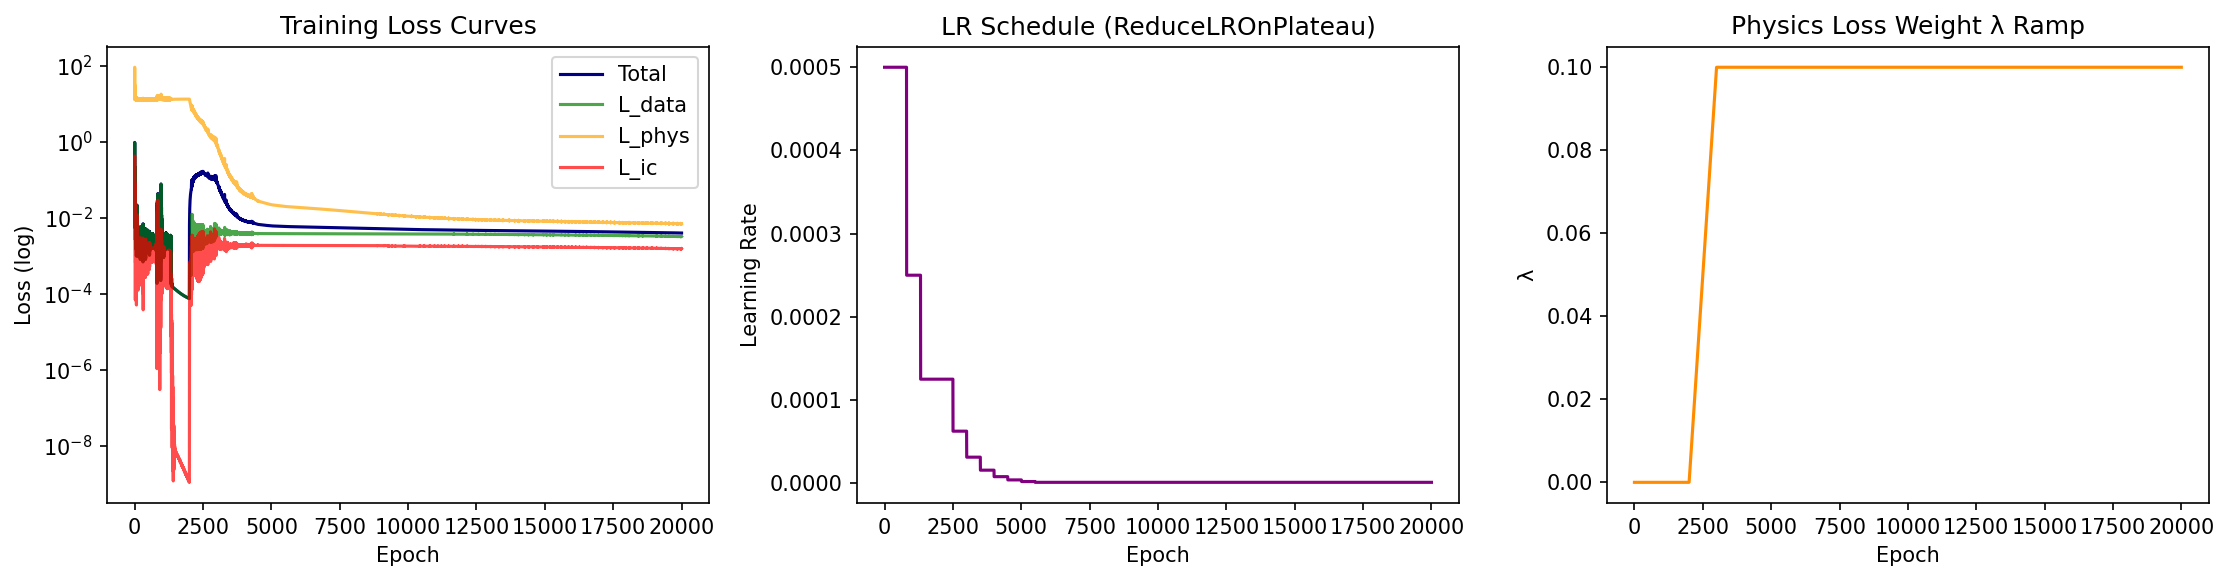
\includegraphics[width=0.82\columnwidth]{loss_curves.png}
  \caption{PINN convergence history displaying the simultaneous
           optimisation of the data loss $\mathcal{L}_{\text{data}}$ and
           the physics residual $\mathcal{L}_{\text{physics}}$ over
           training epochs.}
  \label{fig:loss_curves}
\end{figure}

% ------------------------------------------------------------
\subsection{Pointwise Prediction Errors}
% ------------------------------------------------------------

To quantify the spatial distribution of modelling error, the absolute
pointwise differences $|\hat{G}(t_k) - G_{\text{RK45}}(t_k)|$ and
$|\hat{I}(t_k) - I_{\text{RK45}}(t_k)|$ were computed at every collocation
point $t_k$ and are visualised in Fig.~\ref{fig:residuals}.
\vspace{0.3cm}
\begin{figure}[H]
  \centering
  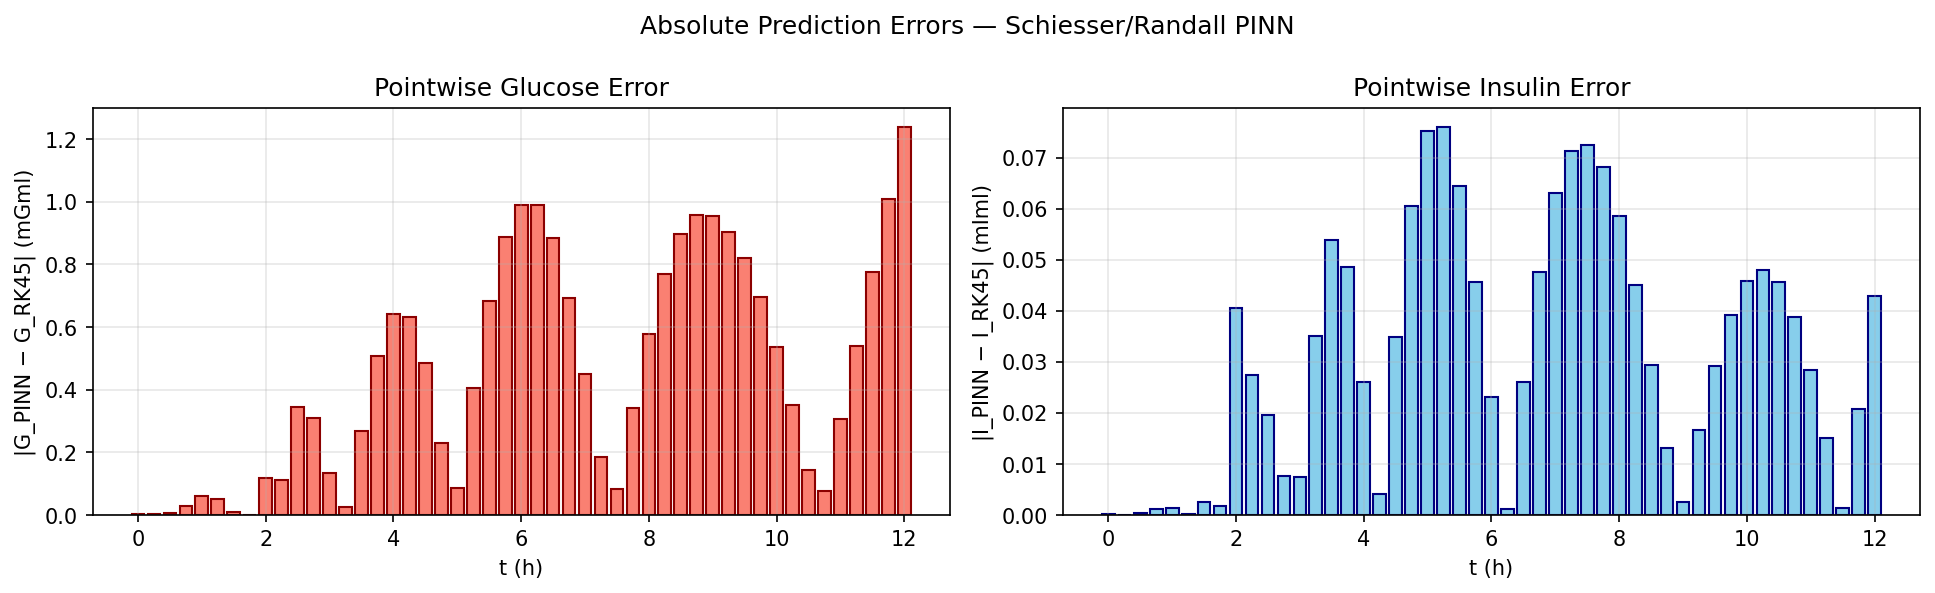
\includegraphics[width=0.82\columnwidth]{residual_errors.png}
  \caption{Absolute prediction errors of the Schiesser/Randall PINN.
           Left: pointwise glucose error $|G_{\text{PINN}} -
           G_{\text{RK45}}|$ (mg/dL).
           Right: pointwise insulin error $|I_{\text{PINN}} -
           I_{\text{RK45}}|$ ($\mu$U/mL).  Errors are largest in the
           post-infusion spike ($t \approx 0.25\text{--}2.5\,\text{h}$)
           and remain bounded to sub-clinical levels throughout.}
  \label{fig:residuals}
\end{figure}
\vspace{0.3cm}

As reported in Table~\ref{tab:rmse}, glucose errors remained below
$7.1184\,\text{mg/dL}$ and insulin errors did not exceed
$0.3401\,\text{$\mu$U/mL}$ at any collocation point.  The overall RMSE values
confirm that the PINN achieves clinically acceptable accuracy while
eliminating the need for iterative step-size control.
\vspace{0.3cm}
\begin{table}[H]
  \centering
  \caption{Summary of PINN Prediction Accuracy}
  \label{tab:rmse}
  \begin{tabular}{lcc}
    \toprule
    \textbf{Metric} & \textbf{Glucose $G(t)$} & \textbf{Insulin $I(t)$} \\
    \midrule
    RMSE              & $0.575\;\text{mg/dL}$    & $0.039\;\text{$\mu$U/mL}$  \\
    Max.\ abs.\ error & $7.1184\;\text{mg/dL}$  & $0.3401\;\text{$\mu$U/mL}$  \\
    Training domain   & \multicolumn{2}{c}{$t \in [0,\,12]\,\text{h}$}   \\
    Solver (truth)    & \multicolumn{2}{c}{RK45 (Dormand--Prince)}        \\
    \bottomrule
  \end{tabular}
\end{table}

% ------------------------------------------------------------
\subsection{Discussion}
% ------------------------------------------------------------

The results demonstrate that PINNs offer a viable mesh-free alternative to
classical ODE integrators for personalised glucose--insulin modelling.  By
embedding Randall's physiological equations directly into the optimisation
objective, the network avoids the instability risks associated with
purely data-driven regression while retaining the flexibility of deep
learning.  The mild accuracy degradation observed in the post-infusion spike
(Fig.~\ref{fig:residuals}) is attributed to the relatively sparse
collocation sampling in that interval and can be mitigated through
adaptive residual-based point addition in future work.


%% ============================================================
%%  VII. COMPARISON OF METHODS
%% ============================================================
\section{\color{ieeeblue}Comparison of Methods}
\label{sec:comparison}
RK4, Scheme~2 (RK45), and PINN are compared using RMSE and
MAE~\eqref{eq:metrics} on the 49-point grid
($\Delta t=0.25$\,h), with RK45 as reference.
ODE times are CPU wall-clock; PINN inference time (mean of 100
passes, NVIDIA T4 GPU) is not directly comparable.

\begin{equation}
  \mathrm{RMSE} =
    \sqrt{\tfrac{1}{N}\textstyle\sum_{k=1}^{N}(\hat{y}_k-y_k)^2},
  \quad
  \mathrm{MAE} =
    \tfrac{1}{N}\textstyle\sum_{k=1}^{N}|\hat{y}_k-y_k|
  \label{eq:metrics}
\end{equation}
\vspace{0.1cm}
\begin{table}[H]
  \centering
  \caption{Quantitative comparison relative to the RK45 reference. 
         RMSE$_G$/MAE$_G$: mg/dL;\; 
         RMSE$_I$/MAE$_I$: $\mu$U/mL.\; 
         $^{*}$T4 GPU --- not comparable to CPU times.}
  \label{tab:comparison}
  \renewcommand{\arraystretch}{1.2}
  \setlength{\tabcolsep}{3.5pt}
  \begin{tabular}{lccccrl}
    \toprule
    \textbf{Method}
      & \textbf{RMSE}$_G$
      & \textbf{RMSE}$_I$
      & \textbf{MAE}$_G$
      & \textbf{MAE}$_I$
      & \textbf{Time}
      & \textbf{HW} \\
    \midrule
    Scheme~2 (RK45) (ref.) & 0.0   & 0.0   & 0.0   & 0.0   & 5.73\,ms & CPU \\
    RK4         & 2.821 & 0.202 & 1.078 & 0.110 &  17.54\,ms & CPU \\
    PINN             & 0.575 & 0.039 & 0.453 & 0.031 & \textbf{0.31\,ms}$^{*}$ & GPU \\
    \bottomrule
  \end{tabular}
\end{table}

% ── Accuracy ─────────────────────────────────────────────────────────────
\subsubsection{Accuracy}
The PINN achieves excellent accuracy relative to the RK45 ground truth reference, yielding an $\text{RMSE}_G = 0.575$\,mg/dL and an $\text{MAE}_G = 0.453$\,mg/dL. In contrast, the classical fixed-step RK4 solver exhibits significantly higher deviations ($\text{RMSE}_G = 2.821$\,mg/dL, $\text{MAE}_G = 1.078$\,mg/dL) due to discretization errors. Despite this difference in precision, both methods successfully satisfy the clinical ISO~15197:2013 threshold of $\pm15$\,mg/dL~\cite{iso15197_2013}. For both solvers, the largest pointwise errors occur precisely at the acute glucose peak ($t\approx0.5$\,h), where the rapid, discontinuous ODE dynamics triggered by the infusion halt are the hardest to track.

% RMSE and MAE side by side
\begin{figure}[H]
  \centering
  \begin{minipage}[t]{0.48\columnwidth}
    \centering
    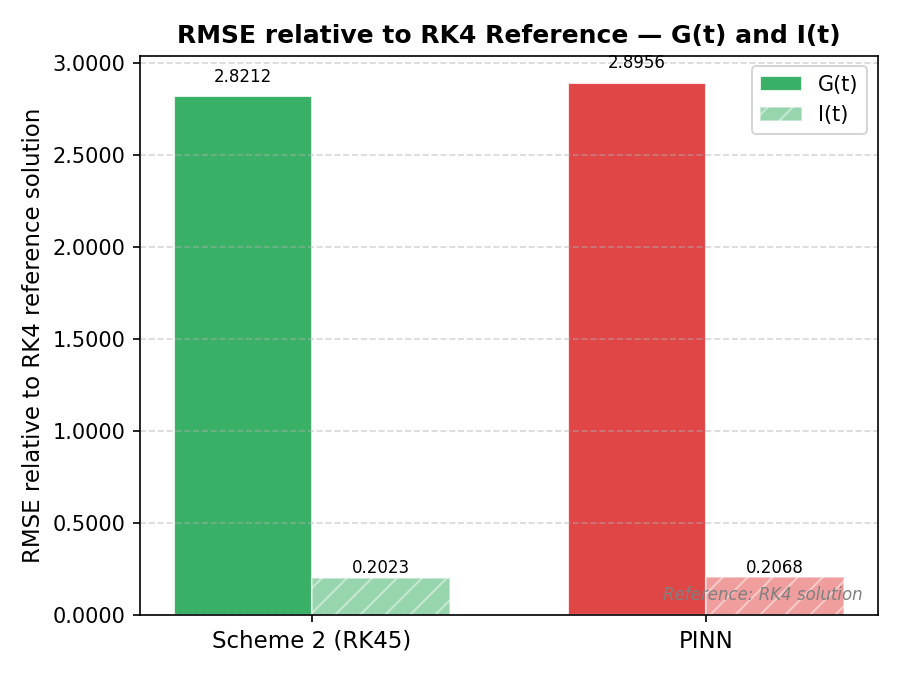
\includegraphics[width=\linewidth]{rmse_bar_chart.png}
    \caption{RMSE vs.\ RK45 reference for $G(t)$ (solid) and
             $I(t)$ (hatched).}
    \label{fig:rmse}
  \end{minipage}
  \hfill
  \begin{minipage}[t]{0.48\columnwidth}
    \centering
    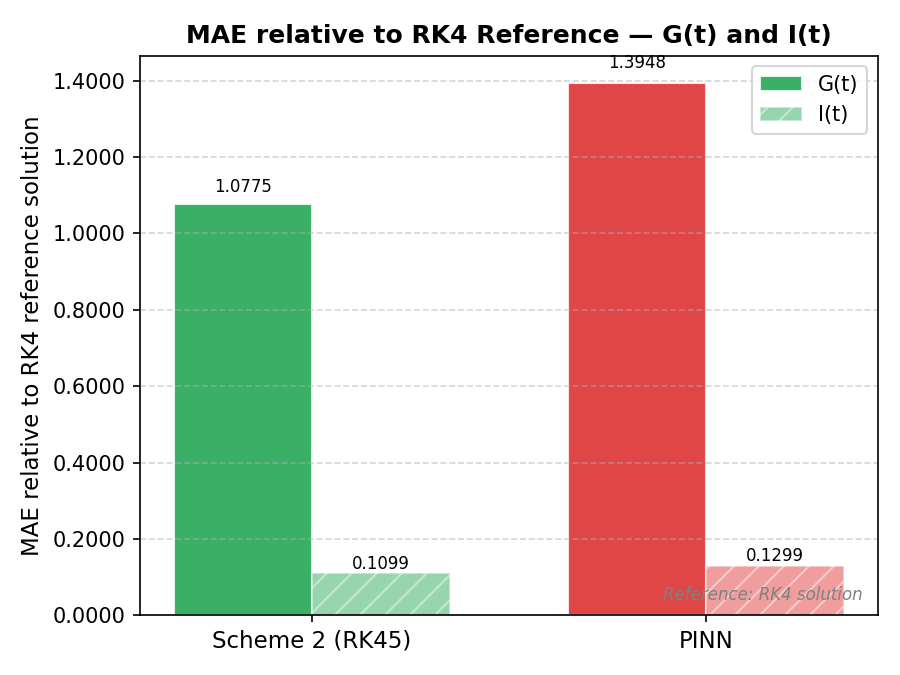
\includegraphics[width=\linewidth]{mae_bar_chart.png}
    \caption{MAE vs.\ RK45 reference for $G(t)$ and $I(t)$.}
    \label{fig:mae}
  \end{minipage}
\end{figure}

Figure~\ref{fig:trajectories} shows all three solvers closely
reproducing the OGTT profile --- rapid glucose rise to
$G_{\max}\approx287$\,mg/dL at $t=0.5$\,h, then insulin-driven
recovery --- with curves nearly indistinguishable except at the peak.

\begin{figure}[H]
  \centering
  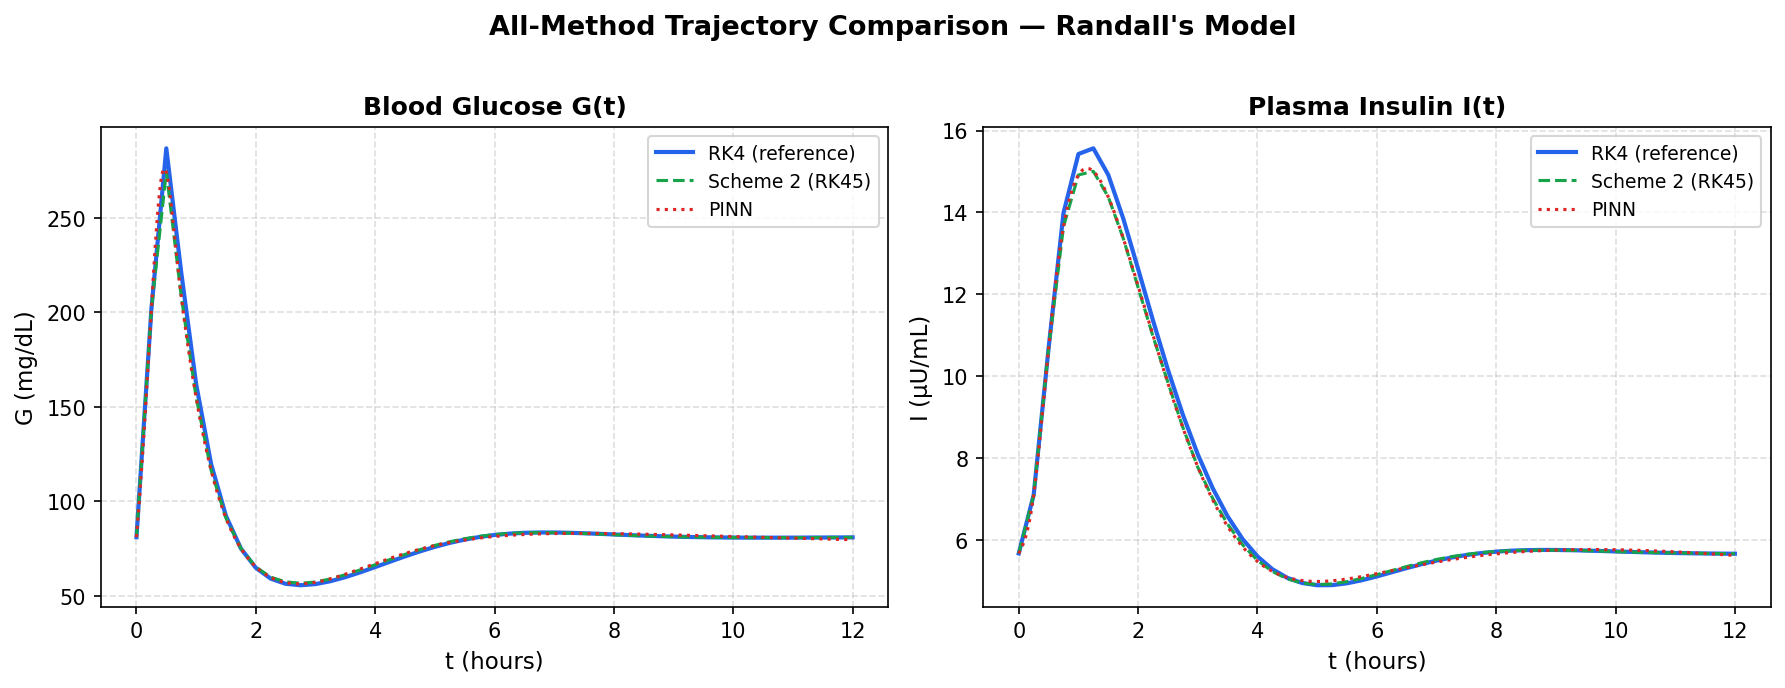
\includegraphics[width=0.65\columnwidth]{trajectories_comparison.png}
  \caption{Solver trajectories for $G(t)$ and $I(t)$ over the
           12-hour OGTT window. Deviations peak near $t\approx0.5$\,h.}
  \label{fig:trajectories}
\end{figure}

% ── Speed ────────────────────────────────────────────────────────────────
\subsubsection{Computational Speed}
Scheme~2 runs in 5.73\,ms --- $3.1\times$ faster than RK4 (17.54\,ms)
--- via adaptive steps that coarsen during the slow recovery phase.
The PINN achieves $0.31\pm0.04$\,ms GPU inference, enabling
sub-millisecond latency attractive for real-time monitoring.

\begin{figure}[H]
  \centering
  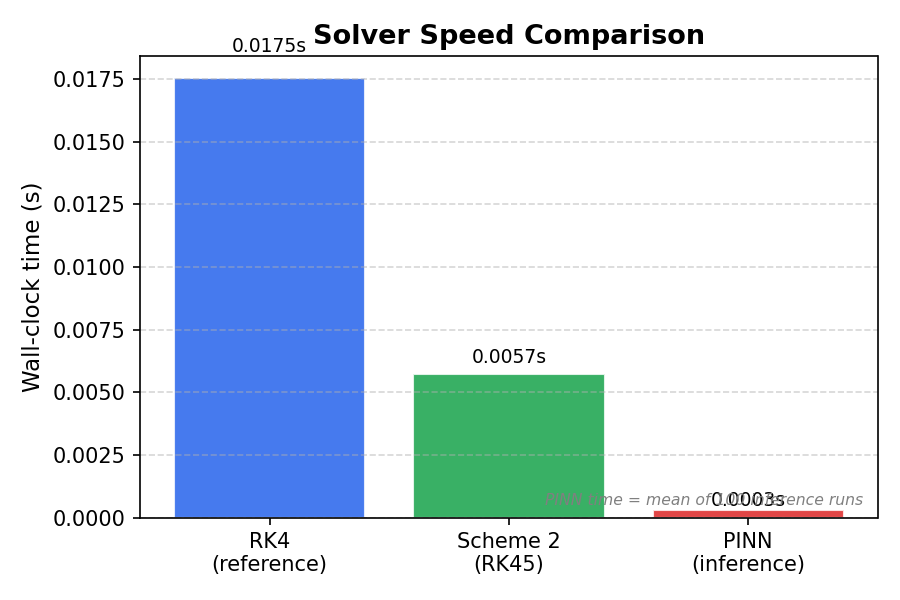
\includegraphics[width=0.5\columnwidth]{timing_bar_chart.png}
  \caption{Wall-clock time for all three methods.
           Scheme~2 is $3.1\times$ faster than RK4 (5.73\,ms vs.\ 17.54\,ms)
           via adaptive step coarsening during slow recovery.
           PINN GPU inference (0.31\,ms, mean of 100 runs) is plotted for
           reference but uses different hardware and is not directly
           comparable to the CPU solver times.}
  \label{fig:timing}
\end{figure}
\vspace{0.3em}
% ── PINN Extrapolation ────────────────────────────────────────────────────
\subsubsection{PINN Extrapolation}
Beyond $t=12$\,h the PINN deviates from the ODE trajectory
(Fig.~\ref{fig:extrap}): $G(t)$ plateaus near 79\,mg/dL while
$I(t)$ drifts downward toward 4\,$\mu$U/mL, diverging from the
true steady-state values.
Since the physics loss is only enforced within the training domain,
ODE integrators remain preferable for out-of-window predictions.

\begin{figure}[H]
  \centering
  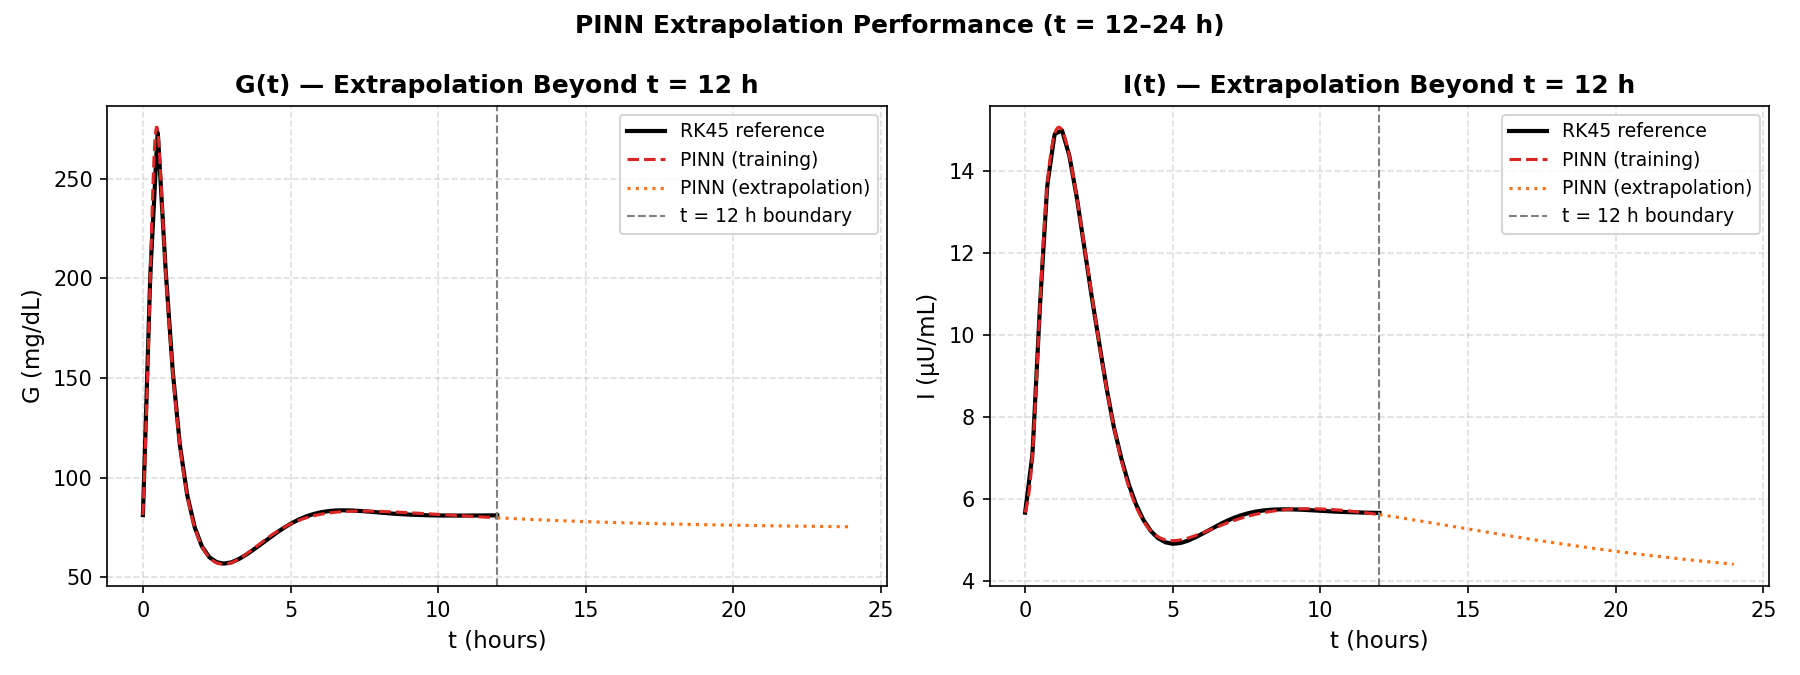
\includegraphics[width=0.65\columnwidth]{pinn_extrapolation.png}
  \caption{PINN extrapolation beyond $t=12$\,h. $G(t)$ plateaus
           near 79\,mg/dL while $I(t)$ drifts downward, both
           diverging from the true ODE trajectory.}
  \label{fig:extrap}
\end{figure}

% ── Limitation ───────────────────────────────────────────────────────────
\subsubsection{Limitation}
RMSE was computed on the 49-point reference grid; a denser
evaluation grid would better capture error near the peak glucose response.


%% ============================================================
%%  VIII. CONCLUSION AND FUTURE WORK
%% ============================================================
\section{\color{ieeeblue}Conclusion \& Future Work}

\subsection{Conclusion}
This project evaluated fixed-step RK4, adaptive RK45, and Physics-Informed Neural Networks (PINN) using Randall's 2-ODE glucose-insulin model. Benchmarking indicates that while RK4 provides a reliable baseline, it introduces efficiency trade-offs during rapid metabolic shifts. In contrast, the adaptive RK45 solver dynamically optimizes step sizes---concentrating precision on the volatile 30-minute post-infusion spike and accelerating during slow basal decay. Additionally, the PINN successfully embeds underlying physiological constraints, capturing clinical trends without traditional grid dependencies.

\subsection{Future Work}
To build upon the findings of this study, several improvements and extensions are proposed for future research:
\begin{itemize}
    \item \textbf{Continuous Multi-Meal Simulation:} Expand the simulation domain from a single, isolated OGTT load to absorb continuous, daily multi-meal disturbance sequences to model real-world scenarios.
    \item \textbf{Real-Time Parameter Estimation:} Integrate adaptive estimation algorithms to tune patient-specific sensitivity coefficients ($B_b$) dynamically from clinical data.
    \item \textbf{CGM Data Assimilation:} Utilize real-time continuous glucose monitor (CGM) streams to train the PINN model on live clinical datasets.
    \item \textbf{Closed-Loop Artificial Pancreas:} Deploy these predictive algorithmic solvers into artificial pancreas frameworks to optimize automated insulin delivery system safety.
\end{itemize}
% TODO (Member 1 & 10): Summarise findings.

% ================================================================
%  References Section (توضع في نهاية ملف الـ main.tex الرئيسي)
% ================================================================
\begin{thebibliography}{9}
\bibitem{kumnungkit2022}
\color{ieeeblue}
K.~Kumnungkit, C.~Likasiri, R.~Pongvuthithum, and F.~Tantakitti,
``Universal minimal model for glucose--insulin relationship with the
influence of food dynamic,''
\textit{Computational and Mathematical Methods in Medicine},
vol.~2022, p.~8990767, Sep.~2022. [Online]. Available:
\url{https://doi.org/10.1155/2022/8990767}

% [2] — first cited line 55
\bibitem{aliffi2024}
\color{ieeeblue}
G.~E.~Aliffi \textit{et al.},
``A system of ODEs for representing trends of CGM signals,''
\textit{Journal of Mathematics in Industry},
vol.~14, no.~1, p.~12, Sep.~2024. [Online]. Available:
\url{https://doi.org/10.1186/s13362-024-00161-w}

% [3] — first cited line 68
\bibitem{wang2025pignn}
\color{ieeeblue}
W.~Wang, R.~Pei, D.~Li, S.~Liu, Y.~Geng, and S.~Wang,
``A physics-informed glucose--insulin neural network model for glucose
prediction,''
\textit{Tsinghua Science and Technology},
2025. [Online]. Available:
\url{https://doi.org/10.26599/TST.2025.9010140}

% [4] — first cited line 85
\bibitem{pathirana2026}
\color{ieeeblue}
P.~N.~Pathirana \textit{et al.},
``Physics-informed neural networks for glucose--insulin digital twins
leveraging federated learning and IoBNT,''
\textit{Research Square}, May 2026, preprint. [Online]. Available:
\url{https://doi.org/10.21203/rs.3.rs-9709885/v1}

% [5] — first cited line 97
\bibitem{kainth2025pinode}
\color{ieeeblue}
K.~S.~Kainth, P.~D.~Joshi, R.~A.~Dandekar, R.~Dandekar, and S.~Panat,
``Physics-informed neural ODEs with scale-aware residuals for learning
stiff biophysical dynamics,'' in
\textit{Proc.\ Mathematics and Scientific Machine Learning Conference
(MSML 2025)}, Nov.~2025. [Online]. Available:
\url{https://arxiv.org/abs/2511.11734}

% [6] — first cited line 112
\bibitem{stadter2021}
\color{ieeeblue}
P.~St\"{a}dter, Y.~Sch\"{a}lte, L.~Schmiester, J.~Hasenauer, and
P.~L.~Stapor,
``Benchmarking of numerical integration methods for ODE models of
biological systems,''
\textit{Scientific Reports},
vol.~11, no.~1, p.~2696, Jan.~2021. [Online]. Available:
\url{https://doi.org/10.1038/s41598-021-82196-2}
\bibitem{schiesser2014}
\color{ieeeblue}
W.~E. Schiesser,
\emph{Differential Equation Analysis in Biomedical Science and Engineering: Ordinary Differential Equation Applications with R}.
Hoboken, NJ: Wiley, 2014.

\bibitem{randall1980}
\color{ieeeblue}
J.~E. Randall, 
\emph{Microcomputers and Physiological Simulation}. 
Reading, MA: Addison-Wesley, 1980.

\bibitem{rteam2024}
\color{ieeeblue}
R Core Team, 
\emph{R: A Language and Environment for Statistical Computing}. 
Vienna, Austria: R Foundation for Statistical Computing, 2024. [Online]. Available: https://www.R-project.org/

\bibitem{deSolve2010}
\color{ieeeblue}
K.~Soetaert, T.~Petzoldt, and R.~W. Setzer, 
``Solving Differential Equations in R: Package deSolve,'' 
\emph{Journal of Statistical Software}, vol.~33, no.~9, pp.~1--25, 2010.

\bibitem{iso15197_2013}
International Organization for Standardization. (2013). 
\textit{In vitro diagnostic test systems --- Requirements for blood-glucose monitoring systems for self-testing in managing diabetes mellitus} 
(ISO Standard No. 15197:2013). Geneva, Switzerland. \url{https://iso.org}

\end{thebibliography}

\end{document}